\chapter{Konzept}
\label{sec:konzept}
Im Konzept wird beschrieben, wie die Problemstellung, welch im \cref{sec:einleitung:ziel} aufgezeigt wurde, gelöst werden kann. Dazu werden zuerst die einzusetzenden Algorithmen evaluiert (siehe \cref{sec:konzept:disziplin-und-algorithmen} \nameref{sec:konzept:disziplin-und-algorithmen}) und aufgezeigt, wie diese angewendet werden (siehe \cref{sec:konzept:anwendungderalgorithmen} \nameref{sec:konzept:anwendungderalgorithmen}). Anschliessend werden die Daten beschrieben und deren Vorbereitung erläutert (siehe \cref{sec:recherche:datenbestand} \nameref{sec:recherche:datenbestand}). \todo{ergänzen 4.4-4.6}

\section{Selektion der Disziplinen und Algorithmenen}
\label{sec:konzept:disziplin-und-algorithmen}
Im \cref{sec:recherche} wurden Disziplinen und Algorithmen erläutert. In diesem Abschnitt wird erklärt wie diese Auswahl getroffen wurde auf Basis der Anforderungen aus \cref{sec:anforderungsanalyse}.

\subsection{Einschränkung der Data Mining Disziplinen}
\label{sec:konzept:disziplinauswahl}
Ziel dieser Arbeit ist es, Attribute von Objekten zu eruieren, welche in einer Gruppe von Buchungen oft vorkommen (siehe \cref{sec:einleitung:ziel} \nameref{sec:einleitung:ziel}). Nachfolgend wird anhand dieser Aufgabenstellungen entschieden, welche Disziplinen im Data Mining (siehe \cref{sec:recherche:dataminingtechniken:disziplinen} \nameref{sec:recherche:dataminingtechniken:disziplinen}) sich dazu eignen. Als Grundlage der Entscheidung gelten die gestellten Anforderungen welche in der Anforderungsanalyse definiert wurden (siehe \cref{sec:anforderungsanalyse:funktionaleanforderung} \nameref{sec:anforderungsanalyse:funktionaleanforderung}).


\subsubsection{Association rule learning}
\label{sec:konzept:disziplinauswahl:association}
Mittels Association rule learning (siehe \cref{sec:recherche:dataminingtechniken:disziplinen:association} \nameref{sec:recherche:dataminingtechniken:disziplinen:association}) lassen sich aus allen selektierten Buchungen die Häufigkeiten von Attributkombinationen herausfinden. Dadurch können FA1, FA2, FA3 sowie FA4 erfüllt werden.


\subsubsection{Classification}
\label{sec:konzept:disziplinauswahl:classification}
Bei der Classification handelt es sich um ein \gls{supervisedlearning} (siehe \cref{sec:recherche:dataminingtechniken:disziplinen:classification} \nameref{sec:recherche:dataminingtechniken:disziplinen:classification}). Deshalb sind vorab Klassen zu definieren welche den Objekten zugewiesen werden. Diese Informationen sind jedoch noch nicht vorhanden, weshalb in der Anforderung FA7 ein \gls{unsupervisedlearning} Algorithmus vorausgesetzt wurde. Deshalb eignet sich die Classification für diese Aufgabenstellung nicht.

\subsubsection{Lineare Regression}
\label{sec:konzept:disziplinauswahl:regression}
Linere Regression Algorithmen suchen eine Formel, damit man von einer abhängiger Variable auf unabhängige Grössen schliessen kann (siehe \cref{sec:recherche:dataminingtechniken:disziplinen:regression} \nameref{sec:recherche:dataminingtechniken:disziplinen:regression}). Dadurch können Attribute vorhergesagt werden. Zum Beispiel wenn man die Kreditwürdigkeit von Kunden überprüfen möchte auf Basis von bestehenden Buchungen. Oder am Beispiel von Interhome ob ein Kunde eher ein Objekt in Italien oder in der Schweiz buchen wird. Obwohl das sicherlich auch interessant ist, eignet sich dieser Algorithmus nicht um die funktionalen Anforderungen zu erfüllen.

\subsubsection{Cluster analysis}
\label{sec:konzept:disziplinauswahl:clusteranalysis}
Das Resultat einer Cluster analysis sind Gruppen (Clusters) von Buchungen, die untereinander ähnlich, und zu allen anderen Gruppen möglichst unähnlich sind (siehe \cref{sec:recherche:dataminingtechniken:disziplinen:clusteranalysis} \nameref{sec:recherche:dataminingtechniken:disziplinen:clusteranalysis}). Zum Beispiel können bei den Interhome Gruppen von Kunden ermittelt werden, welche ähnliche Kaufverhalten aufweisen. 

Obwohl das Clustering keine funktionale Anforderung beantwortet, ist der Ansatz trotzdem interessant. Da die Instanzen innerhalb des Clusters ähnlich zueinander sind ist zu erwarten, dass eine Häufigkeitszählung der Attribute innerhalb des Clusters ähnliche Eigenschaften aufweisen. Diese sollten von der Apriori Analyse gefunden werden. 

Dies könnte hilfreich sein, wenn über die gesamte zu analysierende Datenmenge die Attributverteilung sehr gleichmässig ist und das Association rule learning keine interessanten Kenntnisse liefert. Das schliesst nicht aus, das es zwei Gruppen gibt, welche für sich selber betrachtet sehr eindeutige Attributverteilungen besitzen, die sich aber gegenseitig aufheben. Zum Beispiel könnte es in Malta viele junge Besucher geben, welche kleine und günstige Ferienhäuser buchen um dort Parties zu feiern. Gleichzeitig gibt es viele Familien die dort hingehen und ausserhalb der Feierzone Strandferien machen. Über alles betrachtet könnte es sein, dass sich die beiden Gruppen aufheben, aber jede für sich selber betrachtet interessante Muster beinhalten aufweisen würde.

Deshalb wird ein versucht gewagt mittels der Cluster analysis zuerst eine Gruppierung der Buchungen durchzuführen, mit einem anschliessenden Association rule learning.

\subsubsection{Collaborative Filtering}
\label{sec:konzept:disziplinauswahl:collaborativefiltering}
Collaborative Filtering werden für recommender systems eingesetzt um dem Benutzer Instanzen vorzuschlagen, die er auch mögen könnte. Grundlage für diese Entscheidungen sind seine bisherigen Interaktionen mit dem System, verglichen mit denen von anderen Benutzern. Dadurch könnte bei den Interhome Daten Objekte vorgeschlagen werden die der Kunde auch mögen könnte. Es werden jedoch keine Attribute vorgeschlagen, womit keine funktionalen Anforderungen erfüllt wird.

\subsection{Algorithmenauswahl}
\label{sec:konzept:algorithmenauswahl}
Im \cref{sec:konzept:disziplinauswahl} wurden die Disziplinen auf Association rule learning und Cluster analysis eingeschränkt und im \cref{sec:recherche:algorithmen} die einzusetzenden Algorithmen beschrieben. Nachfolgend wird aufgezeigt, wieso jene Techniken gewählt wurden.

\subsubsection{Association rule learning: Apriori}
\label{sec:konzept:algorithmenauswahl:apriori}
Das Association rule learning besteht aus zwei Schritten. Zuerst werden mittels des Apriori Algorithmus häufige Attributkombinationen gesucht und anschliessend Regeln aufgestellt, um Korrelationen zwischen gemeinsam auftretenden Eigenschaften aufzuzeigen.
In dieser Arbeit wird nur der Apriori Algorithmus implementiert. Dieser erlaubt es FA1, FA2, FA3 und FA4 zu beantworten. Der zweite Schritt wird nicht durchgeführt, da die Regeln des Association rule learning für die Aufgabenstellung dieser Arbeit nicht benötigt werden.

Es gibt Alternativen zum Apriori Algorithmus. Dies sind zum Beispiel der AprioriTid oder AprioriHybrid. Diese generieren die identischen Resultate und unterscheiden sich nur in der Laufzeit. Der AprioriTid kann zu beginn der Häufigkeitszählung bessere Leistung aufzeigen, ist jedoch langsamer gegen dessen Ende. Der AprioriHybrid verwendet zu Beginn der Apriori, und am Schluss den AprioriTid\footcite{association_rule_learning_2017-01-05}. 

Es ist noch unklar, welcher Algorithmus die besseren Laufzeiten aufweist. Zum Schluss oder nach der Arbeit kann in einer Vertiefung der AprioriTid oder der AprioriHybrid eingesetzt werden um die Leistungen der Algorithmen zu vergleichen. Im ersten Schritt wird der Apriori benutzt um zu analysieren, ob die Resultate brauchbare Informationen liefern.

\subsubsection{Clustering}
\label{sec:konzept:algorithmenauswahl:clustering}
Es gibt diverse Algorithmen welche sich verschiedene Problemstellungen annehmen. Unterteilen lassen sich diese in vier Gruppen:
\begin{itemize}
	\item Partitioning
	\item Hierarchical
	\item Density-based
	\item Grid-mased
\end{itemize}
Nicht alle Algorithmen lassen sich eindeutig einer Gruppe zuweisen. Jedoch hilft diese Auflistung eine Übersicht über die Verfahren zu geben\footcite{data_mining_concepts_and_techniques}.

Für die Auswahl eines Algorithmus müssen die Charakteristiken der Daten bekannt sein, wie diese zum Beispiel verteilt (z.B. Kugel-, Kreis-, S-Förmig) oder wie viele Cluster sinnvoll sind. Diese sind bislang jedoch noch bekannt.
Partitioning- und Hierarchical-Vorgehensweisen benötigen zur Berechnung der Clustern deren Anzahl. Bei ersteren kann diese anhand der Elbow-Methode berechnet werden\footcite{elbow_method}. Bei Hierarchischen Clustern müsste man dies jedoch für jeden Ast ermittelt. Da die Laufzeit von solchen Algorithmen bereits $\mathcal{O}(k^2)$ beträgt ist diese Vorgehensweise nicht praktikabel\footcite{complexity_hierarchical_clustering} (siehe \cref{sec:anforderungsanalyse:algorithmen:komplexitaet} \nameref{sec:anforderungsanalyse:algorithmen:komplexitaet}). Grid-based Methoden unterteilen den Datenraum in ein Netz wodurch die Clusters erzeugt werden. Unterstützt werden dabei nur numerische Daten weshalb sich diese Gruppe nicht eignet (weitere Forschung in dem Bereich ist jedoch im Gange\footcite{sting_categorical_data}).
Aus diesen Gründen werden in dieser Arbeit ein Vertreter aus der Partitioning (k-prototype) und der Density-based (DBSCAN) Gruppen umgesetzt.

\paragraph{k-prototypes als partitionierender Algorithmus}
\label{sec:konzept:algorithmenauswahl:clustering:kprototypes}
Bei den partitionierenden Algorithmen sind die bekanntesten Vertreter der k-means und der k-medoids. Beide funktionieren nur mit numerischen Daten, weshalb eine alternative mit dem k-prototypes eruiert wurde. Der k-prototypes ist eine Abwandlung vom k-medoids und wurde im \cref{sec:recherche:algorithmen:k-prototypes} beschrieben. Dieser Algorithmus wurde gewählt, da er mit numerischen, sowie mit kategorischen Daten umgehen kann und mit Medoiden anstelle vom geometrischer Schwerpunkt arbeitet. Letzteres hat den Vorteil, dass der Algorithmus damit robuster gegenüber Ausreissern ist\footcite{data_mining_concepts_and_techniques}. Ob es Ausreisser in den Interhome Daten gibt ist noch unbekannt. Es ist jedoch zu erwarten, dass es einige exotische Objekte gibt, die selten gebucht werden und das Clustering damit verziehen. 

\paragraph{DBSCAN als density-based Algorithmus}
\label{sec:konzept:algorithmenauswahl:clustering:dbscan}
Als Vertreter der Density-based Algorithmen wird \gls{dbscan} verwendet. Beschrieben der er im \cref{sec:recherche:algorithmen:dbscan}. Als alternative bietet sich \gls{optics} an. Dabei handelt es sich um eine Erweiterung von \gls{dbscan}, bei welchem kein Dichte $\epsilon$ angegeben werden muss. Jedoch erstellt \gls{optics} keine Clusters, sondern eine geordnete aufsteigende Liste, sodass räumlich benachbarte Punkte in dieser Ordnung nahe aufeinander liegen. Die Auswertung der Liste muss nachgelagert ausgeführt werden\footcite{data_mining_concepts_and_techniques}. In dieser Arbeit wird \gls{dbscan} verwendet da mit geeigneten, noch zu ermittelnden, werten für $\epsilon$ und $minpts$ ein Clustering erstellt werden kann und der Benutzer die Resultate nicht noch weiter interpretieren muss. Sollte es nötig sein, so kann nach der Arbeit überprüft werden ob \gls{optics} bessere Resultate liefert.

\section{Anwendung der Algorithmen}
\label{sec:konzept:anwendungderalgorithmen}
Bei der Anwendung der Algorithmen gibt es Probleme, welche in diesem Abschnitt beschrieben werden. Zum einen müssen die Algorithmen vergleichbar sein, wozu eine einheitliche Distanzmessung eingesetzt wird und sie müssen mit kategorischen Attributen arbeiten können. Diese Problematik wird im \cref{sec:konzept:anwendungderalgorithmen:distanzmessung} näher erläutert. Zum anderen müssen die verschiedenen Parameter, welche die Algorithmen benötigen, korrekt gesetzt werden, was im \cref{sec:konzept:parameterauswahl} besprochen wird.

\subsection{Distanzmessung}
\label{sec:konzept:anwendungderalgorithmen:distanzmessung}
Um die Resultate der Clustering Algorithmen zu vergleichen wird eine einheitliche Funktion $d$ zur Distanzmessung definiert.
Dazu eignet sich zum Beispiel die quadratische euklidische Distanz wie sie in der \cref{eq:recherche:clusteranalysis:1} aufgezeigt wird.

\begin{equation} \label{eq:recherche:clusteranalysis:1}
d(I_i, I_j) = \sum_{k=1}^{m} (A_{ik} - A_{jk})^2
\end{equation}

$A_{ik}$ ist das k-te Attribute der Instanz $i$. 
Diese Distanzmessung eignet sich nur für numerische Attribute.
Da die Interhome Daten jedoch hauptsächlich aus kategorischen Attirbuten bestehen, wird  eine erweiterte Funktion zur Messung der Entfernung verwendet, welche im Artikel zum k-prototype Algorithmus von Zhexue Huang vorgeschlagen wird\footcite{clustering_numeric_and_categorical_values}.
Dabei handelt es sich um eine Fusion der quadratischen euklidischen- und der Hamming-Distanz\footcite{data_mining_concepts_and_techniques}.

\begin{equation} \label{eq:recherche:clusteranalysis:2}
d(I_i, I_j) = \sum_{k=1}^{m} (A^n_{ik} - A^n_{jk})^2 + \gamma \sum_{k=1}^{m} \delta(A^c_{ik}, A^c_{jk})
\end{equation}

$A^n_{ik}$ und $A^c_{ik}$ stehen für die numerischen ($A^n$) beziehungsweise kategorischen ($A^c$) Attribute $k$ der Instanz $i$. 
$\gamma$ ist das Gewicht mit welcher die numerischen und kategorischen Attribute verglichen werden.
$\delta$ ist definiert als:

\begin{equation} \label{eq:recherche:clusteranalysis:3}
\delta(p,q)= 
\begin{cases}
1,				& \text{if } p \neq q\\
0,              & \text{otherwise}
\end{cases}
\end{equation}

Dadurch erhalten Instanzen mit vielen Übereinstimmungen eine kleinere Distanz als wenn Attribute unterschiedliche Werte aufweisen.

\subsection{Parameterauswahl}
\label{sec:konzept:parameterauswahl}
Für die Clustering Algorithmen und die Distanzmessung werden Eingabeparameter benötigt, dessen Auswahl in diesem Abschnitt erläutert wird.

Für \gls{dbscan} wird $\epsilon$ und $minpts$ benötigt, sowie $\gamma$ für die Distanzmessung (siehe \cref{sec:recherche:algorithmen:dbscan} \nameref{sec:recherche:algorithmen:dbscan} sowie \cref{sec:konzept:anwendungderalgorithmen:distanzmessung} \nameref{sec:konzept:anwendungderalgorithmen:distanzmessung}). Diese Werte müssen explorativ ermittelt werden. Dazu werden im \cref{sec:recherche:testcases} Testcases definiert welche Clusters beinhaltet. Die Parameter müssen so gesetzt werden, dass die vordefinierten Clusters gefunden werden. Anschliessend können die selben Werte auf den produktiven Daten angewendet werden.

Die Ermittlung des $k$ Wertes beim k-prototypes Algorithmus wird im \cref{sec:konzept:parameterauswahl:kprototypes} beschrieben.

\subsubsection{k Auswahl für k-prototypes}
\label{sec:konzept:parameterauswahl:kprototypes}
Der k-prototypes benötigt die Anzahl an Clustern $k$ die generiert werden sollen. Zu Beginn ist jedoch noch unklar wie dieser Parameter gewählt werden soll. Mithilfe der Elbow-Methode kann der optimale Wert für $k$ ermittelt werden. Dazu wird der Algorithmus mit einem Cluster durchgeführt und danach der Wert um jeweils 1 erhöht. Der Gesamtfehler des Clusterings (total within-cluster variation) wird schlussendlich über alle Werte für $k$ in ein Koordinatensystem eingetragen. Dies ergibt eine Kurve wie sie in \cref{fig:konzept:parameterauswahl:kprototypes} aufgezeigt wird.

\begin{figure}[H]
	\RawFloats
	\centering
	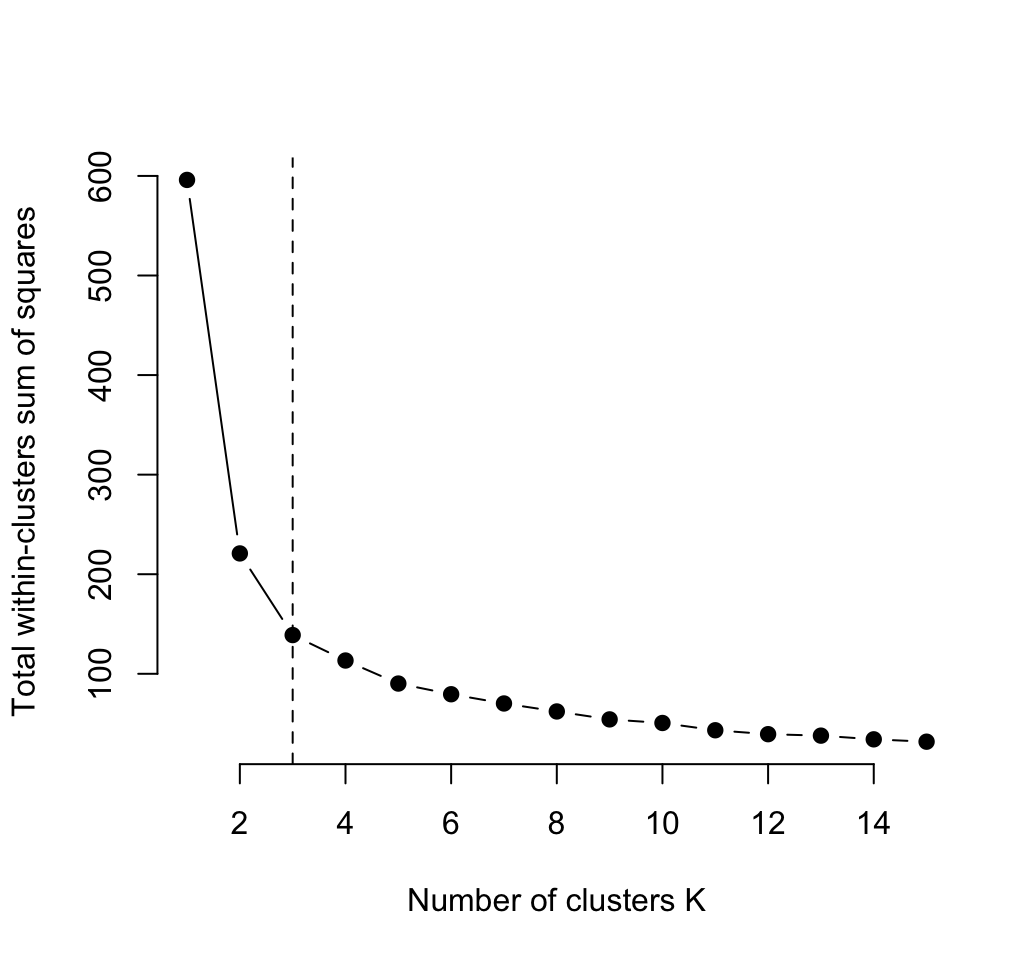
\includegraphics[width=0.8\textwidth]{images/elbow-curve.png}
	\caption{Elbow-Kurve}
	\source{\cite{elbow_method}}
	\label{fig:konzept:parameterauswahl:kprototypes}
\end{figure}

Bei einem Cluster $k=1$ ist der Fehler am grössten und erreichen 0 wenn $k=n$, wobei $n$ die Anzahl Instanzen darstellt. Der optimale Wert liegt dort wo die Kurve beginnt abzuflachen. Im obigen Beispiel ist dies $k=3$.

\section{Datenbestand}
\label{sec:recherche:datenbestand}
Nachfolgend wird der Datenbestand und die selektion der Attribute erklärt.

\subsection{Beschreibung der Daten}
\label{sec:recherche:datenbeschaffung}
Die Daten für die Auswertung wurden aus dem \gls{irent} extrahiert werden. Da die Buchungen Kundendaten enthalten, können sie nicht veröffentlicht werden.

Die Daten liegen im Windows Excel Format vor. Es sind total 133'001 Datensätze mit jeweils 153 Felder. Die Felbeschreibungen sind im \cref{app:feldbeschreibungen} aufgeführt. Zellen A-U sind Informationen im Bezug auf die Buchungen, alle anderen (V-EW) beziehen sich auf das Objekt selber.

"`boolean"' Datentypen werden behandelt wie "`categorical"' Werte mit nur zwei Ausprägungen, sprich "`0"' und "`1"',

\subsection{Datenvorbereitung}
\label{sec:recherche:datenvorbereitung}
Die Datenvorbereitung wandelt die Daten so um dass sie für das Data Mining möglichst effizient verwendet werden können. Dies umfasst die Bereinigung, Transformation sowie Reduktion von Informationen\footcite{feature_selection_2017-01-04}. Bei ersteren werden Messfehler im Datenbestand behoben, fehlende Felder ergänzt oder Duplikate entfernt. Die Transformation wandelt Werte um damit sie für die Berechnung besser geeignet sind. Zum Beispiel können Wertebereiche in Intervalle aufgeteilt werden. Bei letzteren werden Instanzen der Datengrundlage entfernt, wodurch die Berechnungszeit verkürzt wird, oder Attribute von allen Instanzen entfernt, da deren Entropie zu gering ist. Zum Beispiel ist es unspannend, wenn ein Attribut bei (fast) allen Instanzen gleich ist. 

\subsubsection{Boolsche Werte}  
\label{sec:recherche:datenvorbereitung:boolschewerte}
In der Datenbasis sind boolsche Werte entweder leer oder "`X"'. Dies wird umgewandelt auf "`0"' oder "`1"'.

\subsubsection{Filtrieren von stornierten Buchungen}
\label{sec:recherche:datenvorbereitung:filtrieren}
Die Datenbasis beinhaltet bestätigte und stornierte Buchungen. Der Status wird in der Zeile C BOOKSTA gespeichert und besitzt den Wert "`OK"' wenn der Kunde die Rechnung bezahlt sowie die Reise angetreten ist, sonst beinhaltet das Feld die Buchstaben "`XX"'. Gründe für eine Stornierung gibt es viele. Zum Beispiel wenn er falsch gebucht hat, die Rechnung nicht bezahlte, die Reise nicht angetreten werden konnte, etc. Wenn es eine ernsthafte Buchung war könnte man auch annullierte Instanzen verwenden in der Analyse. Wenn jedoch etwas falsch gebucht wurde könnten diese Buchungen die Analyse verfälschen. Da kein Grund für die Annullierung angegeben ist in der Datenbasis werden alle Instanzen mit "`XX"' entfernt. 

\subsubsection{Datennormierung von numerischen Werten} 
\label{sec:recherche:datenvorbereitung:normierung} \cref{sec:konzept:anwendungderalgorithmen:distanzmessung} vorgestellte Distanzmessung arbeitet mit der euklidischen Distanz für numerische Werte. Wenn ein Attribut $A_1$ einer Buchung den Wert 1'000 hat und das einer anderen Buchung 300, so ergibt sich eine Distanz von 700. Betrachtet man ein anderes Attribut $A_2$, welches den Wert 1 hat beziehungsweise 0.3, so ist die Distanz 0.7. Dadurch fällt $A_2$ in der gesamten Distanz zwischen den beiden Buchungen überhaupt nicht in Gewicht, da es um einen Faktor 1'000 kleiner ist. Deshalb werden numerische Attribute genormt, damit alle in den gleichen Wertebereich liegen.

In dieser Arbeit werden vier numerische Attribute verwendet.
\begin{table}[H] 
	\caption{Numerishce Attribute}
	\centering
	\rowcolors{1}{tablebodycolor}{tablerowcolor}
	\label{fig:recherche:datenvorbereitung:5}
	\begin{tabular}{ | c | c | c | l | } 
		\hline 
		\rowcolor{tableheadcolor}
		\bfseries Zelle & \bfseries Name & \bfseries Datentyp & \bfseries Beschreibung \\ \hline 
		E & PRICES & integer & Preis \\ \hline 
		AC & QUAL & integer & Sterne Bewertung des Objektes \\ \hline 
		AD & ROOMS & integer & Anzahl Zimmer \\ \hline 
		AE & BEDROOMS & integer & Anzahl Schlafzimmer \\ \hline 
	\end{tabular}
\end{table}

Normiert werden die Spalten AC (Sterne Bewertung des Objektes), AD (Anzahl Zimmer) und AE (Anzahl Schlafzimmer). Diese werden in ein Intervall zwischen 0 und 1 überführt.

Der Preis in der Spalte E giltet für die gesamte Buchung. Dieser wird in einen Wochenpreis und pro Person normiert. Wenn eine Buchung CHF 2'000 kostet für 10 Tage für 2 Personen, so ergibt das "`CHF 1'400 / 10 Tage * 7 Tage / 2 Personen = CHF 490"'. Es wird keine Normierung auf einen Wert von 0-1 durchgeführt, da dieser Wert noch diskretiert wird (siehe nächsten Paragraphen).

\subsubsection{Datenerweiterung} 
Die Daten sollen durch weitere Felder ergänzt werden. Denn eine Fragestellung von Interhome ist es, eine Häufigkeitsanalyse in einem Gebiet durchzuführen\todo{cref}. Da im Datenstamm jedoch nur das Land des Objektes vorhanden ist, muss die Region und die Ortschaft erweitert werden. 

Zusätzlich müssen für die Wetterdaten die genaue Geolocation des Benutzers vorhanden sein. Im Datenstamm ist die Adresse des Kunden gespeichert, mit welcher die Geolocation ermittelt werden kann.

\subsubsection{Diskretierung von Distanzen und des Wochenpreises} 
\label{sec:recherche:datenvorbereitung:diskretierung}
Die Zeilen AK (Distanz zum Wasser), AL (Distanz zum Skigebiet), AM (Distanz zum öffentlichen Verkehr), DZ (Distanz zum Zentrum), EA (Distanz bis zum Meer) und EB (Distanz bis zum See) sind numerische Werte, welche die Anzahl an Metern zu einem Punkt angeben. Die Werte dieser Spalten wird in folgenden Wert diskretiert. 

\begin{table}[h] 
	\caption{Diskretisierungswerte für Distanzattribute}
	\centering
	\rowcolors{1}{tablebodycolor}{tablerowcolor}
	\label{fig:recherche:datenvorbereitung:1}
	\begin{tabular}{ | c | c | c | } 
		\hline 
		\rowcolor{tableheadcolor}
		\bfseries Min & \bfseries Max & \bfseries Wert \\ \hline 
		0 & 499 & close \\ \hline 
		500 & $\infty$ &   \\ \hline 
	\end{tabular}
\end{table}

Ebenfalls wird der Wochenpreise in nachfolgende Intervalle unterteilt.
\begin{table}[h] 
	\caption{Diskretisierungswerte des Preises}
	\centering
	\rowcolors{1}{tablebodycolor}{tablerowcolor}
	\label{fig:recherche:datenvorbereitung:2}
	\begin{tabular}{ | c | c | c | } 
		\hline 
		\rowcolor{tableheadcolor}
		\bfseries Min & \bfseries Max & \bfseries Wert \\ \hline 
		0 & 200 & budget \\ \hline 
		201 & 400 &  \\ \hline 
		401 & $\infty$ & luxury \\ \hline 
	\end{tabular}
\end{table}

Bei den Distanzen sind kleine Werte spannend, welche angeben dass ein Objekt nahe am Skilift oder bei der Busstation liegt. Deshalb wurde definiert dass die Werte von 0 bis 499 Metern als nahe (engl. Close) markiert werden. Darüber liegende Werte werden ignoriert.

Bei den Preisen hingegen ist es interessant, wenn ein Objekt besonders günstig oder teuer ist. Deshalb wurden zwei Intervalle definiert. Nämlich 0 bis 200 und 401 aufwärts. Alles dazwischen wird nicht weiter behandelt.

Diese Datenreduktion wird vorgenommen, da dadurch die Informationen auch von der Apriori-Analyse verwendet werden kann. Diese zählt nur exakte Übereinstimmungen. Sprich zwei Objekte, welche CHF 1 auseinander liegen wären gleich unterschiedlich als wenn deren Unterschied CHF 1'000 beträge.

Die Schwellwerte der diskretierungen wurden mit Interhome abgesprochen.

\begin{itemize}
%\item Das Datenformat wurde für die einfachere programmatische Handhabung von Windows Excel in das \gls{csv}-Format transferiert.
\item Boolsche Werte ist entweder leer (gleichbedeutend mit "`0"') oder "`X"' (gleichbedeutend mit "`1"'). Die Werte werden geändert auf 0 und 1.
\item Distanzen in den Zeilen AK (Distanz zum Wasser), AL (Distanz zum Skigebiet), AM (Distanz zum öffentlichen Verkehr), DZ (Distanz zum Zentrum), EA (Distanz bis zum Meer) und EB (Distanz bis zum See) werden diskretisiert. Dabei interessiert es Interhome nur, wenn die Nähe kleiner als 500 ist. Alles über oder gleich 500 wird nicht verwendet. Siehe \cref{fig:recherche:datenvorbereitung:1}.
\item Der Preis wird normiert auf Wochenpreise. wurde diskretisiert. Spannend für die Interpretation sind nur werte welche kleiner als 500 sind oder über 2000. Siehe \cref{fig:recherche:datenvorbereitung:2}.
\end{itemize}

In den Tabellen \ref{fig:recherche:datenvorbereitung:3} und \ref{fig:recherche:datenvorbereitung:4} wird ein Beispiel gegeben. In der ersten Tabelle sind Buchungen vor der diskretisierung aufgeführt und in der zweiten danach. Distanzwerte von 500 oder mehr und Preise zwischen 499 und 2000 wurden entfernt. Dies ist zum Beispiel bei dem Wert "`Distanz zum Skilift"' der Buchung mit ID 3 geschehen.

\begin{table}[H] 
	\caption{Datenbestand vor der Diskretisierung}
	\centering
	\rowcolors{1}{tablebodycolor}{tablerowcolor}
	\label{fig:recherche:datenvorbereitung:3}
	\begin{tabular}{ | c | c | c | c | c | c | c | c | } 
		\hline 		
		\rowcolor{tableheadcolor}
		\bfseries \rotatebox{90}{ID} & \bfseries \rotatebox{90}{Ortschaft} & \bfseries \rotatebox{90}{Preis (CHF)} & \bfseries \rotatebox{90}{Tiere erlaubt} & \bfseries \rotatebox{90}{Grill vorhanden} & \bfseries \rotatebox{90}{Balkon vorhanden} & \bfseries \rotatebox{90}{Distanz zum Meer (m)} & \bfseries \rotatebox{90}{Distanz zum Skilift (m)} \\ \hline 
		
		1 & Zermatt & 230 & \checkmark &  &  &  & 150 \\ \hline 
		2 & Cannes & 450 & & \checkmark & \checkmark & 260 & \\ \hline 
		3 & Zermatt & 2301 & \checkmark & \checkmark & & 350 & 850 \\ \hline 
		4 & Zermatt & 879 & \checkmark & & \checkmark &  & 350 \\ \hline 
		5 & Zermatt & 149 & \checkmark &  & \checkmark &  & 450 \\
		6 & Cannes & 873 &  & \checkmark &  & 80 & 1200 \\ \hline 
		7 & Zermatt & 1800 & \checkmark & \checkmark &  & 760 & \\ \hline 
	\end{tabular}
\end{table}

\begin{table}[H] 
	\caption{Datenbestand nach der Diskretisierung}
	\centering
	\rowcolors{1}{tablebodycolor}{tablerowcolor}
	\label{fig:recherche:datenvorbereitung:4}
	\begin{tabular}{ | c | c | c | c | c | c | c | c | } 
		\hline 		
		\rowcolor{tableheadcolor}
		\bfseries \rotatebox{90}{ID} & \bfseries \rotatebox{90}{Ortschaft} & \bfseries \rotatebox{90}{Preis} & \bfseries \rotatebox{90}{Tiere erlaubt} & \bfseries \rotatebox{90}{Grill vorhanden} & \bfseries \rotatebox{90}{Balkon vorhanden} & \bfseries \rotatebox{90}{Distanz zum Meer (m)} & \bfseries \rotatebox{90}{Distanz zum Skilift (m)} \\ \hline 
		
		1 & Zermatt & budget & \checkmark &  &  &  & close \\ \hline 
		2 & Cannes & budget & & \checkmark & \checkmark & close & \\ \hline 
		3 & Zermatt & luxury & \checkmark & \checkmark &  & close & \\ \hline 
		4 & Zermatt &  & \checkmark & & \checkmark &  & close \\ \hline 
		5 & Zermatt & budget & \checkmark &  & \checkmark &  & close \\
		6 & Cannes &  &  & \checkmark &  & close &  \\ \hline 
		7 & Zermatt & luxury & \checkmark & \checkmark &  &  & \\ \hline 
	\end{tabular}
\end{table}

Die Diskretisierung wird durchgeführt, damit nach dem Clustering die Häufigkeit der kategorischen Werte mit dem Apriori Algorithmus erhoben werden kann. Dadurch wird das Clustering nachvollziehbar\todo{cref}\footcite{data_mining_concepts_and_techniques}. 

Es gibt verschiedene Diskretisierungsmethoden. Diese Teilen die Werte in gleiche Intervalle auf oder stellen sicher dass in jeder Kategorie die selbe Anzahl an Instanzen vorhanden sind.
Die verwendeten Werte aus \cref{fig:recherche:datenvorbereitung:1} und \cref{fig:recherche:datenvorbereitung:2} wurde mit Interhome abgesprochen. 

\subsection{Attributeinschränkung}
\label{sec:recherche:attributeinschraenkung}
Der Datenbestand besteht aus 153 Attributen/Spalten. Aus folgenden Gründen sollten die Attribute eingeschränkt werden:
\begin{itemize}
\item Laufzeit der Algorithmen kann durch eine Attributreduktion verbessert werden.
\item Es gibt Attribute welche andere Zusammenfassen. In der \cref{fig:recherche:attributeinschraenkung:1} ist die Zelle "`AW"' eine Aggregation von den darunterliegenden Feldern.
\end{itemize}

\begin{table}[H] 
	\caption{Beispiel eines Attributaggregators}
	\centering
	\rowcolors{1}{tablebodycolor}{tablerowcolor}
		\label{fig:recherche:attributeinschraenkung:1}
	\begin{tabular}{ | c | c | c | l | } 
		\hline 
		\rowcolor{tableheadcolor}
		\bfseries Zelle & \bfseries Name & \bfseries Datentyp & \bfseries Beschreibung \\ \hline 
		AW & CPOOL & boolean & Objekt besitzt einen Pool \\ \hline 
		AX & CPPOOL & boolean & Objekt besitzt einen privaten Pool \\ \hline 
		AY & CHEATED & boolean & Objekt besitzt einen geheizten Pool \\ \hline 
		AZ & CSAFEPOOL & boolean & Objekt besitzt einen sicheren Pool \\ \hline 
		BA & CCHILDPOOL & boolean & Objekt besitzt einen kindersicheren Pool \\ \hline 
		DU & OUTDPOOL & boolean & Objekt besitzt einen aussen Pool \\ \hline 
		DV & INDPOOL & boolean & Objekt besitzt einen innen Pool \\ \hline 
	\end{tabular}
\end{table}

In Absprache mit Interhome wurde entschieden, dass in einem ersten Schritt jene Attribute verwendet werden sollen, welche auch direkt auf der Webseite dargestellt werden. Die zu verwendenden Spalten sind in der \cref{fig:recherche:attributeinschraenkung:2} aufgeführt. Das Feld "`NREF"' beinhaltet die Objektidentifikation. Dieses wird für die Attributanalyse nicht verwendet, hilft jedoch den Testern bei der Validierung der Resultate und sollte deshalb beim einsehen des Datenbestandes mit angezeigt werden.

\begin{table}[H] 
	\caption{Zu verwendende Attribute}
	\centering
	\rowcolors{1}{tablebodycolor}{tablerowcolor}
	\label{fig:recherche:attributeinschraenkung:2}
	\begin{tabular}{ | c | c | c | l | } 
		\hline 
		\rowcolor{tableheadcolor}
		\bfseries Zelle & \bfseries Name & \bfseries Datentyp & \bfseries Beschreibung \\ \hline 
		E & PRICES & integer & Preis \\ \hline 
		I & NREF & categorical & Nummer des gebuchten Objektes \\ \hline 
		AC & QUAL & integer & Sterne Bewertung des Objektes \\ \hline 
		AD & ROOMS & integer & Anzahl Zimmer \\ \hline 
		AE & BEDROOMS & integer & Anzahl Schlafzimmer \\ \hline 
		AH & PETS & boolean & Haustiere erlaubt? \\ \hline 
		AK & DIWATER & integer & Distanz zum Wasser (m) \\ \hline 
		AL & DISKI & integer & Distanz zum Skigebiet (m) \\ \hline 
		AM & DIPUBT & integer & Distanz zum öffentlichen Verkehr (m) \\ \hline 
		AR & CAIRCOND & boolean & Aircondition im Objekt\\ \hline 
		AW & CPOOL & boolean & Objekt besitzt einen Pool \\ \hline 
		BC & CBBQ & boolean & Objekt besitzt einen Grill \\ \hline 
		BF & CSAUNA & boolean & Objekt besitzt eine Saune \\ \hline 
		BI & CJACUZZI & boolean & Objekt besitzt ein Jacuzzi \\ \hline 
		BM & CWASHMACHI & boolean & Objekt besitzt eine Waschmaschine \\ \hline 
		BU & CPARKING & boolean & Es gibt einen Parkplatz \\ \hline 
		BV & CDISHWASHE & boolean & Objekt besitzt einen Geschirrspühler \\ \hline
		BW & CFIREPLACE & boolean & Objekt besitzt ein Cheminée \\ \hline 
		BX & SCTV & boolean & Objekt besitzt einen Fernseher \\ \hline  
		BY & SCBALCONY & boolean & Objekt besitzt ein Balkon \\ \hline 
		CA & SCNOSMOKE & boolean & Im Objekt darf nicht geraucht werden \\ \hline 
		DZ & DICENTER & integer & Distanz bis zum Zentrum (m) \\ \hline 
		EA & DISEA & integer & Distanz bis zum Meer (m) \\ \hline 
		EB & DILAKE & integer & Distanz bis zum See (m) \\ \hline 
		EG & INTERNET & boolean & Objekt besitzt Internet \\ \hline 
	\end{tabular}
\end{table}

%Einige Attribute sind mehrfach

\section{Ablauf}
\label{sec:konzept:ablauf}
Der Ablauf des Data Mining im zu entwickelnden Programm ist zweistufig. Als erstes gibt der User eine Abfrage ein, für welche anschliessend eine Liste von häufig auftretenden Attributen gesucht werden soll (siehe \cref{sec:einleitung:ziel} \nameref{sec:einleitung:ziel}).


\subsection{Einschränkung des Datenbestandes}
\label{sec:konzept:ablauf:einschraenkung}
Im ersten Schritt wird der Datenbestand durch die Auswahl von Attributen durch den Benutzer eingeschränkt. Er kann 0-n Werte aus den in der \cref{fig:recherche:attributeinschraenkung:2} gelisteten Attributen selektieren. Anschliessend werden alle Instanzen aus der Datenmenge entfernt welche den Kriterien nicht genügen. Dies bildet die Grundlage für die Analyse im Schritt 2.

\begin{figure}[H]
	\RawFloats
	\centering
	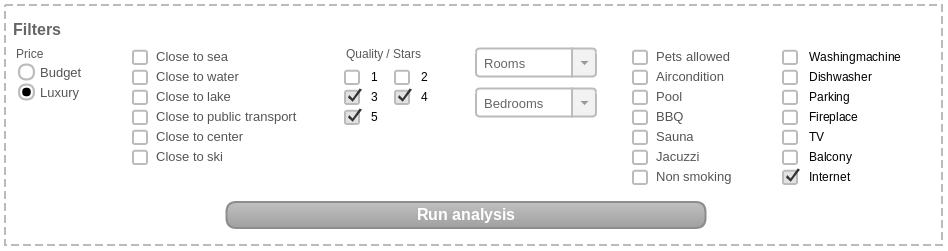
\includegraphics[width=1\textwidth]{images/wireframe-filtering}
	\caption{Mockup für das Filtrieren von Buchungen}
	\label{fig:konzept:ablauf:einschraenkung:1}
\end{figure}

\cref{fig:konzept:ablauf:einschraenkung:1} zeigt einige Filters welche der User auswählen kann. Mit einem Klick auf den "`Run analysis"' Button werden die Daten zuerst eingeschränkt und der Analyseprozess gestartet.

Nach der Einschränkung der Daten werden nur noch folgende Buchungen berücksichtigt, welche den Filtern genügen. \cref{fig:konzept:ablauf:einschraenkung:2} zeigt einen Datenbestand vor der Anwendung von Filtern, und \cref{fig:konzept:ablauf:einschraenkung:3} die Daten danach.
\begin{table}[H] 
	\caption{Datenbestand vor der Anwendung der Filterkriterien}
	\centering
	\rowcolors{1}{tablebodycolor}{tablerowcolor}
	\label{fig:konzept:ablauf:einschraenkung:2}
	\begin{tabular}{ | c | c | c | c | c | c | c | c | c | c |} 
		\hline 		
		\rowcolor{tableheadcolor}
		\bfseries \rotatebox{90}{ID} & \bfseries \rotatebox{90}{Ortschaft} & \bfseries \rotatebox{90}{Preis} & \bfseries \rotatebox{90}{Qualität} & \bfseries \rotatebox{90}{Tiere erlaubt} & \bfseries \rotatebox{90}{Grill vorhanden} & \bfseries \rotatebox{90}{Balkon vorhanden} & \bfseries \rotatebox{90}{Distanz zum Meer (m)} & \bfseries \rotatebox{90}{Distanz zum Skilift (m)} \\ \hline 
		
		1 & Zermatt & budget & 3 & \checkmark &  &  &  & close \\ \hline 
		2 & Cannes & & 3 & & \checkmark & \checkmark & close & \\ \hline 
		3 & Zermatt & luxury & 4 & \checkmark & \checkmark &  & close & \\ \hline 
		4 & Zermatt &  & 4 & \checkmark & & \checkmark &  & close  \\ \hline 
		5 & Zermatt & budget & 2 & \checkmark &  & \checkmark &  & close \\
		6 & Cannes & luxury & 5 &  & \checkmark &  & close &  \\ \hline 
		7 & Zermatt & luxury & 2 & \checkmark & \checkmark &  &  &  \\ \hline 
	\end{tabular}
\end{table}

\begin{table}[H] 
	\caption{Datenbestand nach Anwendung der Filterkriterien}
	\centering
	\rowcolors{1}{tablebodycolor}{tablerowcolor}
	\label{fig:konzept:ablauf:einschraenkung:3}
	\begin{tabular}{ | c | c | c | c | c | c | c | c | c | } 
		\hline 		
		\rowcolor{tableheadcolor}
		\bfseries \rotatebox{90}{ID} & \bfseries \rotatebox{90}{Ortschaft} & \bfseries \rotatebox{90}{Preis} & \bfseries \rotatebox{90}{Qualität} & \bfseries \rotatebox{90}{Tiere erlaubt} & \bfseries \rotatebox{90}{Grill vorhanden} & \bfseries \rotatebox{90}{Balkon vorhanden} & \bfseries \rotatebox{90}{Distanz zum Meer (m)} & \bfseries \rotatebox{90}{Distanz zum Skilift (m)} \\ \hline 
		
		3 & Zermatt & luxury & 4 & \checkmark & \checkmark &  & 350 & \\ \hline 
		6 & Cannes & luxury & 5 &  & \checkmark &  & 80 &  \\ \hline 
	\end{tabular}
\end{table}

\subsection{Auffinden von Attributen}
\label{sec:konzept:ablauf:analyse}
Für den zweiten Schritt wird entweder ein \nameref{sec:konzept:disziplinauswahl:association} (siehe \cref{sec:konzept:disziplinauswahl:association}) oder eine \nameref{sec:konzept:disziplinauswahl:clusteranalysis} (siehe \cref{sec:konzept:disziplinauswahl:clusteranalysis}) durchgeführt. 

Möchte der Benutzer wissen, welche Attribute in der (vorselektierten) Datenmenge oft vorkommen, so kann der Apriori-Algorithmus verwendet werden. Eine beispielhafte Ausgabe ist in der \cref{fig:konzept:ablauf:analyse:1} aufgezeigt. Die erste Tabelle beinhaltet alle einzelnen Attribute welche als häufig erachtet werden, die zweiten Tabelle sind alle häufigen zweier Attributkombinationen, die dritte Tabelle alle dreier Attributkombinationen. Dies geht weiter bis der Apriori-Algorithmus keine häufigen Kombinationen mehr findet.
\begin{figure}[H]
	\RawFloats
	\centering
	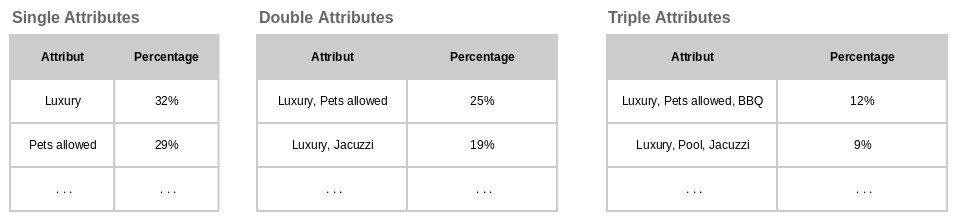
\includegraphics[width=1\textwidth]{images/wireframe-histogram}
	\caption{Auffinden von Attributen}
	\label{fig:konzept:ablauf:analyse:1}
\end{figure}

Liefert der Apriori keine zufriedenstellenden Antworten oder ist von vornherein zu erwarten, dass es verschiedene Gruppen von Buchungen gibt, so kann zuerst die Cluster Analysis durchgeführt werden. Die Instanzen werden damit in Clusters/Klassen aufgeteilt, der Benutzer würde jedoch nicht sehen weshalb. Deshalb wird auf jeder Klasse der Apriori-Algorithmus durchgeführt. Da die Instnzen in einer Klasse untereinander möglichst Homogen sein sollen und möglichst unterschiedlich zu anderen Clusters, ist anzunehmen, dass die häufigsten Attribute, welche durch den Apriori-Algorithmus gefunden werden, aussagekräftig die Klassen beschreiben.

\section{Mockups des Programmes}
\label{sec:konzept:mockups}
Die graphischen Oberfläche des Programmes wird nachfolgend anhand von Mockups aufgezeigt. Die Auflistung der Stammdaten sowie der Resultate ist einfachheitshalber verkürzt dargestellt. Auf jeder Seite zuoberst ist das Interhome Logo sowie die Navigation platziert.

In \cref{fig:konzept:mockups:stammdaten} ist die Startseite abgebildet in welcher der Benutzer die Stammdaten (\nameref{fig:anforderungsanalyse:funktionaleanforderung:fa4}) einsehen kann. Im oberen Bereich sind die Filter, mit welchen der Datenbestand eingeschränkt werden kann. 
\begin{figure}[H]
	\RawFloats
	\centering
	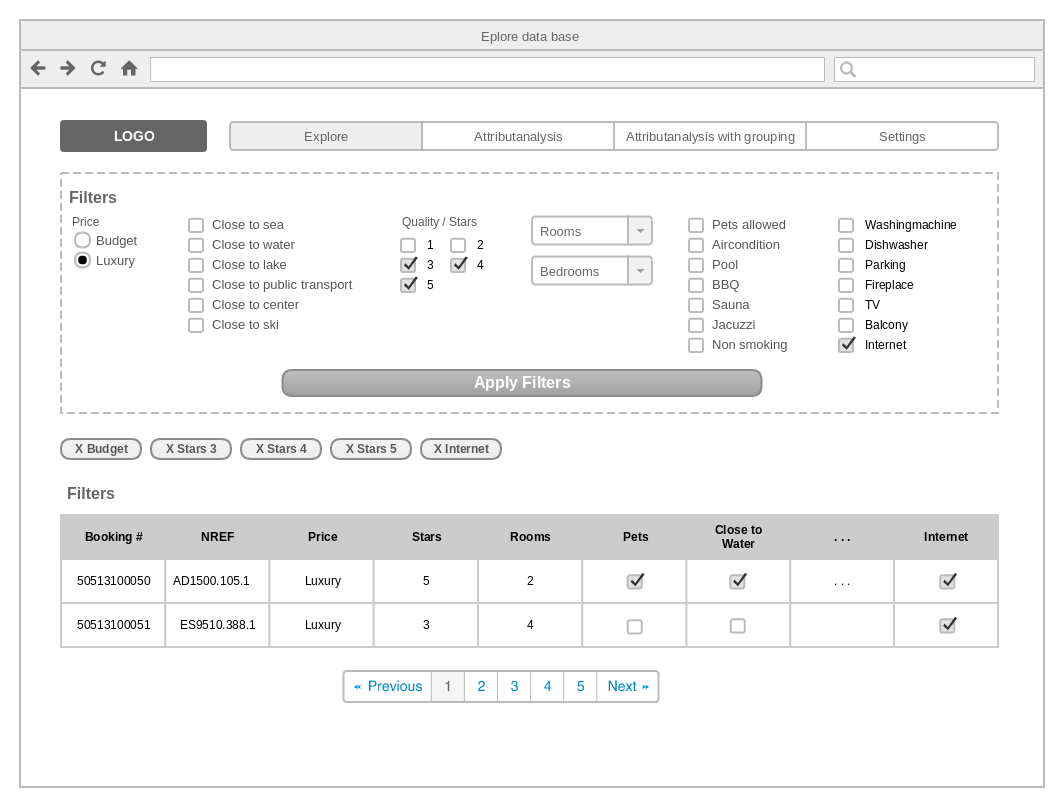
\includegraphics[width=1\textwidth]{images/wireframe-explore}
	\caption{Mockup für das einsehen der Stammdaten (FA4 \& FA5)}
	\label{fig:konzept:mockups:stammdaten}
\end{figure}

Auf der zweiten Seite, welche in \cref{fig:konzept:mockups:apriori} dargestellt ist, kann der Benutzer eine apriori Analyse durchführen (siehe \cref{sec:konzept:algorithmenauswahl:apriori} \nameref{sec:konzept:algorithmenauswahl:apriori}). Wie vorher sind zuoberst die selben Filter platziert. Darunter sind die Attribute aufgelistet, welche vom Algorithmus gefunden wurde sowie deren Häufigkeit. Zuunterst ist zur Kontrolle noch der analysierte Datenbestand aufgeführt.
\begin{figure}[H]
	\RawFloats
	\centering
	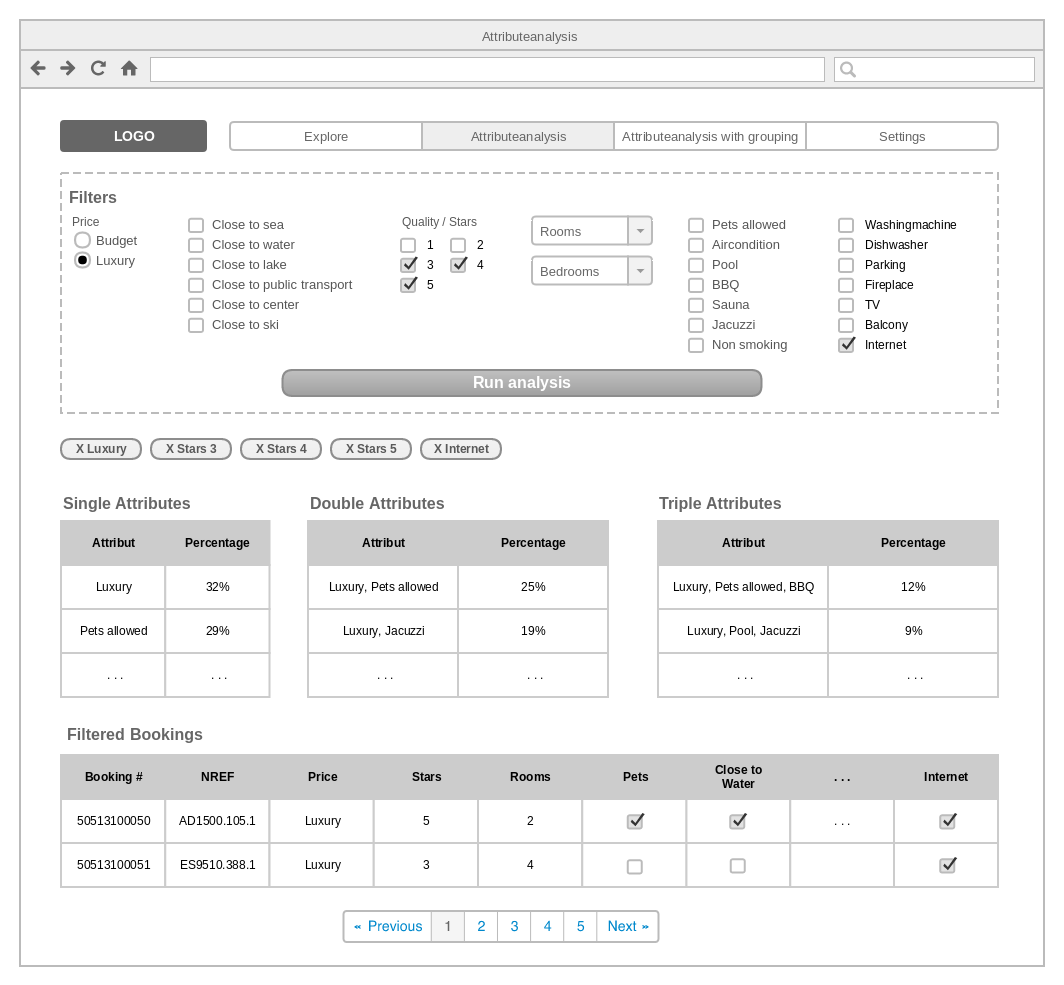
\includegraphics[width=1\textwidth]{images/wireframe-apriori}
	\caption{Mockup für die Analyse mit dem apriori Algorithmus (FA1, FA2 \& FA3)}
	\label{fig:konzept:mockups:apriori}
\end{figure}

Der dritte Reiter führt zur Analyse mit den Clustering Algorithmen k-prototypes und DBSCAN (\cref{sec:konzept:algorithmenauswahl:clustering} \nameref{sec:konzept:algorithmenauswahl:clustering}). Die Filter sind entsprechend den vorherigen Seite zuoberst platziert. Es gibt jedoch zwei Buttons um die Analyse mit den entsprechenden Algorithmen zu starten. Zuunterst sind die gefunden Clusters abgebildet, mit den häufigen Attributen sowie den Buchungen, welche zu den entsprechenden Clustern gehören. Zur Verbesserung der Übersicht können die Bereiche auf- und zugeklappt werden.

\begin{figure}[H]
	\RawFloats
	\centering
	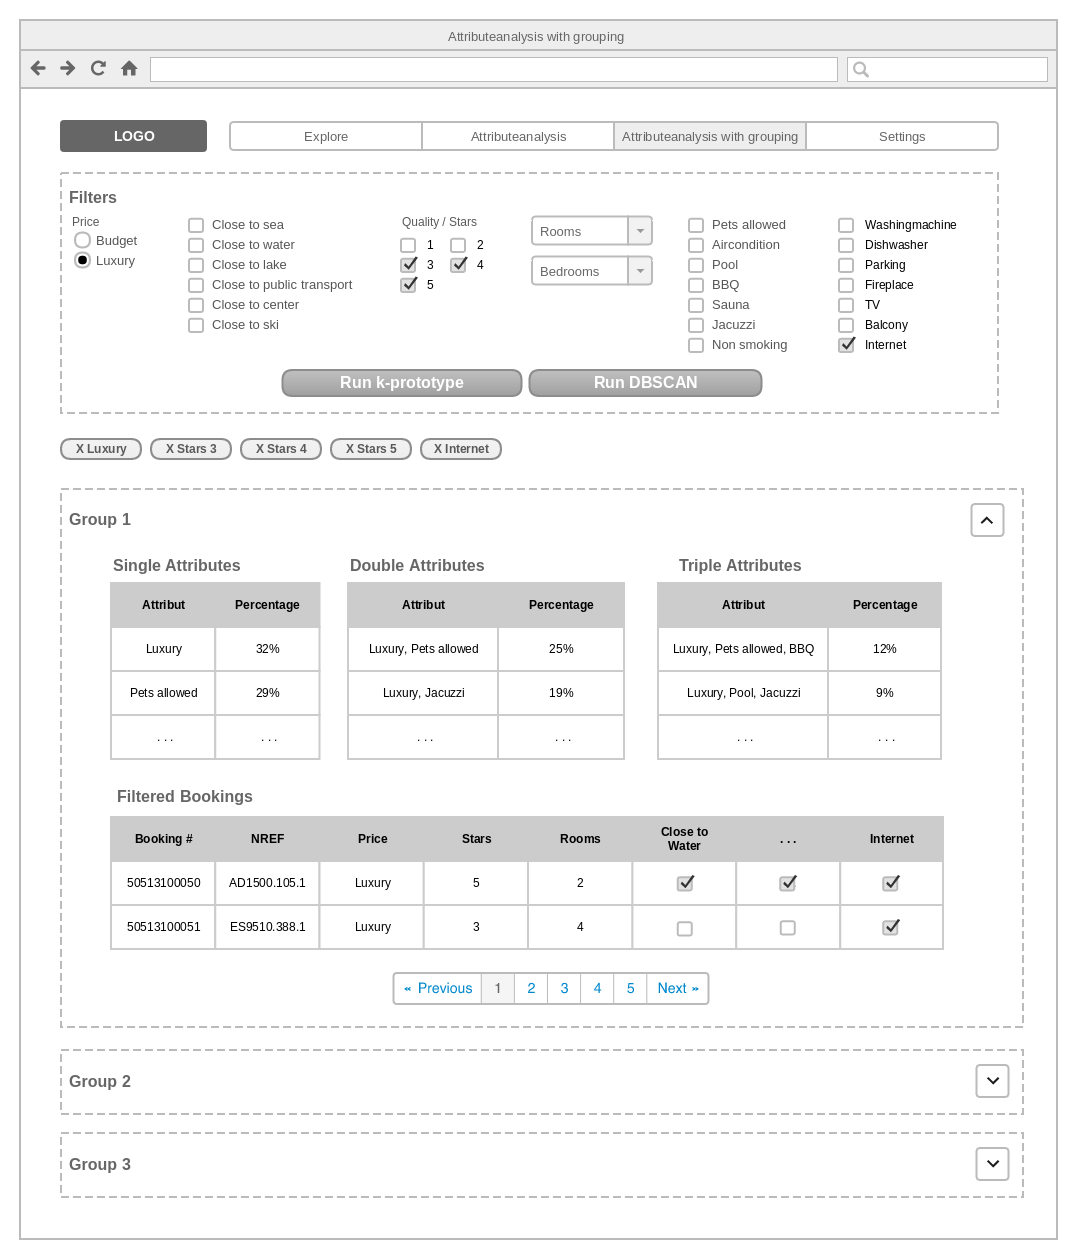
\includegraphics[width=1\textwidth]{images/wireframe-clustering}
	\caption{Mockup für die Analyse mit k-prototpyes und DBSCAN (FA1, FA2 \& FA3)}
	\label{fig:konzept:mockups:clustering}
\end{figure}

Der letzte Mockup zeigt die Ansicht in welcher die Einstellungen des Programmes angepasst werden können. Dabei handelt es sich um ein Formular in welchem jedes Feld eine Einstellungsmöglichkeit darstellt. Zu jedem Wert wird es eine Beschreibung geben damit der Benutzer verstehen kann worum es sich bei dieser Einstellung handelt.

\begin{figure}[H]
	\RawFloats
	\centering
	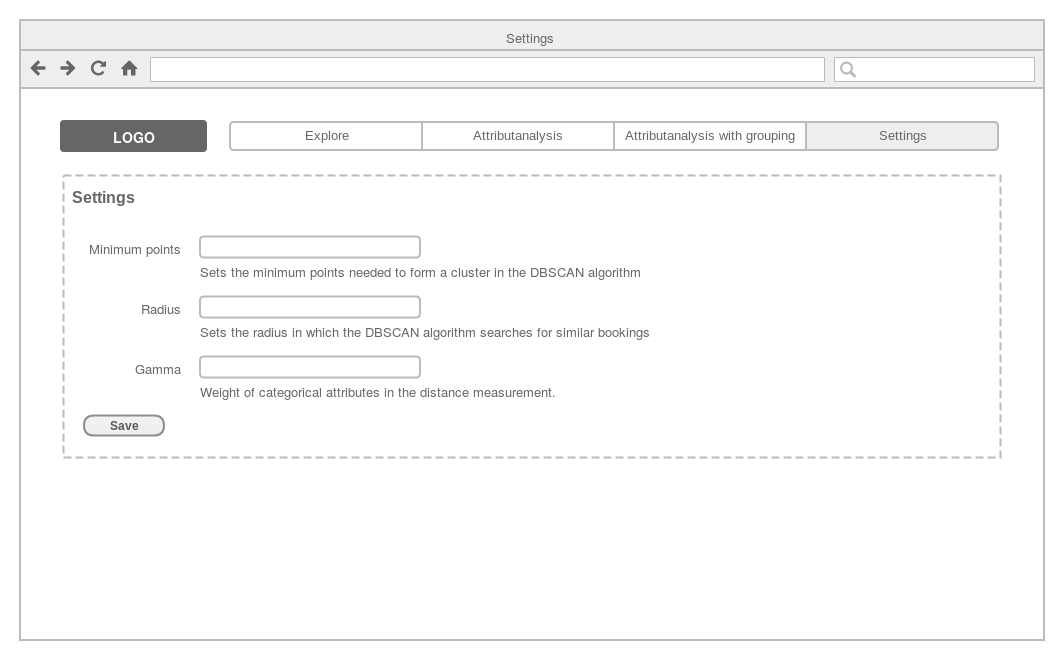
\includegraphics[width=1\textwidth]{images/wireframe-settings}
	\caption{Mockup für die Konfiguration der Algorithmen (FA8)}
	\label{fig:konzept:mockups:settings}
\end{figure}

\section{Testfälle}
\label{sec:recherche:testcases}

% data-apriori-3-entries--2-distances-1-binary.csv
% 17 von 18:
% - Distance water: close
% - Distance see: close
% - Pets allowed: yes
%
% data-apriori-3-entries-two-sets--2-distances--1-number-1-binary.csv
% set 1, 8 von 18:
% - Distance water: close
% - Distance see: close
% set 2, 9 von 18:
% - Rooms: ??? (2?)
% - Pets allowed: yes

In diesem Abschnitt sind Testfälle definiert welche am Schluss der Entwicklung ausgewertet werden (siehe \cref{sec:testingfazit:testing:testcases} \nameref{sec:testingfazit:testing:testcases}). Dadurch können die Erwartungen an das Programm mit der tatsächlichen Ausgabe des Proof of Concepts verglichen werden. Dazu wurden Datenquellen erstellt, in welchen die zu findenden Mustern von vornherein bekannt sind. Sobald der Proof of Concept umgesetzt wurde können die Resultate mit den  nachfolgend vorgestellten Informationen verglichen werden. Dadurch wird die richtige Funktionsweise des Programms sichergestellt.

Es sind 12 Testdatenquellen definiert worden, welche im \cref{app:testdatenquellen} aufgeführt sind.
Sie bestehen aus 9 - 18 Einträge mit jeweils 10 Attributen. Die Felder "`id"' und "`NREF"' in den Quellen sind nur für das Verständnis vorhanden und tragen nicht zur Testauswertung bei. Die restlichen Attribute bestehen aus Distanzen ("`DIWATER"', "`DIPUBT"', "`DISEA"'), Preisen ("`weeklyprice"'), Binär- ("`PETS"', "`CAIRCOND"') und numerischen ("`ROOMS"', "`BEDROOMS"') Werten. Dadurch sind kategorische sowie numerische Attribute abgedeckt. 

Die \glspl{tc} 1 bis 9 überprüfen die Richtigkeit des Apriori Algorithmen. Sie stellen sicher, dass Distanz-, Preis-, binären- und numerischen Attribute richtig aufsummiert und durch den Apriori-Gen Vorgang zu weiteren Attributmengen kombiniert werden. Zusätzlich überprüfen sie ob die Einschränkung der Datenmenge durch den Benutzer korrekt funktionieren. \glspl{tc} 10 bis 12 kontrollieren ihrerseits die Cluster Algorithmen. 

Für die nachfolgenden Erwartungen werden nachfolgende Parameter vorausgesetzt. Diese müssen nachher bei der Testausführung gesetzt werden. Stimmen die Resultate überein ist der Test erfolgreich. 
\begin{itemize}
	\item Apriori
	\begin{itemize}
		\item $minSup$: 3
	\end{itemize}
	
	\item Clustering
	\begin{itemize}
		\item $\gamma$ (Gewicht zwischen numerischen und kategorischen Attributen): 1
		\item k-prototype:
		\begin{itemize}
			\item $k$ (Anzahl an Clustern): 2
		\end{itemize}
		\item DBSCAN:
		\begin{itemize}
			\item $\epsilon$ (Radius): 1
			\item $minpts$ (Minimum Anzahl Punkte im Radius (Prozentwert)): 0.1
		\end{itemize}
	\end{itemize}
\end{itemize}

\paragraph{TC1, Datenquelle \cref{app:testdatenquellen:1}:} Überprüft ob 2 Distanzattribute korrekt aufsummiert und miteinander zu einer 2er Menge kombiniert werden. 

\begin{table}[H] 
	\caption{TC1 Definition}
	\centering
	%\rowcolors{1}{tablebodycolor}{tablerowcolor}
	\label{fig:recherche:testcases:1}
	\begin{tabular}{ | l | l | l | } 
		\hline 
		\rowcolor{tableheadcolor}
		\multicolumn{3}{|l|}{\bfseries ID: TC1} \\ \hline 
		Datebquelle & \multicolumn{2}{|l|}{\cref{app:testdatenquellen:1}} \\ \hline 
		Dateneinschränkung & \multicolumn{2}{|l|}{Keine} \\ \hline 
		
		\rowcolor{tableheadcolor}
		\multicolumn{3}{|l|}{\bfseries Erwartetes Resultat} \\ \hline 
		& Attributmenge & Anzahl \\ \hline 
		
		1er-Attributmenge & \tabitem Nahe am Wasser & 8 \\ \cline{2-3} 
		& \tabitem Nahe am Meer & 8 \\ \hline 
		
		2er-Attributmenge & \tabitem Nahe am Wasser & 8 \\
		& \tabitem Nahe am Meer & \\ \hline
	\end{tabular}
\end{table}

\paragraph{TC2, Datenquelle \cref{app:testdatenquellen:2}:} Überprüft ob 2 Binärattribute korrekt aufsummiert und miteinander zu einer 2er Menge kombiniert werden. 

\begin{table}[H] 
	\caption{TC2 Definition}
	\centering
	\label{fig:recherche:testcases:2}
	\begin{tabular}{ | l | l | l | } 
		\hline 
		\rowcolor{tableheadcolor}
		\multicolumn{3}{|l|}{\bfseries ID: TC2} \\ \hline 
		Datebquelle & \multicolumn{2}{|l|}{\cref{app:testdatenquellen:2}} \\ \hline 
		Dateneinschränkung & \multicolumn{2}{|l|}{Keine} \\ \hline 
		
		\rowcolor{tableheadcolor}
		\multicolumn{3}{|l|}{\bfseries Erwartetes Resultat} \\ \hline 
		& Attributmenge & Anzahl \\ \hline 
		
		1er-Attributmenge & \tabitem Haustiere erlaubt & 8 \\ \cline{2-3} 
		& \tabitem Aircondition vorhanden & 8 \\ \hline 
		
		2er-Attributmenge & \tabitem Haustiere erlaubt & 8 \\
		& \tabitem Aircondition vorhanden & \\ \hline
	\end{tabular}
\end{table}

\paragraph{TC3, Datenquelle \cref{app:testdatenquellen:3}:} Überprüft ob 2 numerische Attribute korrekt aufsummiert und miteinander zu einer 2er Menge kombiniert werden. 


\begin{table}[H] 
	\caption{TC3 Definition}
	\centering
	\label{fig:recherche:testcases:3}
	\begin{tabular}{ | l | l | l | } 
		\hline 
		\rowcolor{tableheadcolor}
		\multicolumn{3}{|l|}{\bfseries ID: TC3} \\ \hline 
		Datebquelle & \multicolumn{2}{|l|}{\cref{app:testdatenquellen:3}} \\ \hline 
		Dateneinschränkung & \multicolumn{2}{|l|}{Keine} \\ \hline 
		
		\rowcolor{tableheadcolor}
		\multicolumn{3}{|l|}{\bfseries Erwartetes Resultat} \\ \hline 
		& Attributmenge & Anzahl \\ \hline 
		
		1er-Attributmenge & \tabitem Anzahl Zimmer=3 & 9 \\ \cline{2-3} 
		& \tabitem Anzahl Schlafzimmer=2 & 9 \\ \hline 
		
		2er-Attributmenge & \tabitem Anzahl Zimmer=3 & 9 \\
		& \tabitem Anzahl Schlafzimmer=2 & \\ \hline
	\end{tabular}
\end{table}

\paragraph{TC4, Datenquelle \cref{app:testdatenquellen:4}:} Überprüft ob 1 numerisches und ein Binärattribut korrekt aufsummiert und miteinander zu einer 2er Menge kombiniert werden.

\begin{table}[H] 
	\caption{TC4 Definition}
	\centering
	\label{fig:recherche:testcases:4}
	\begin{tabular}{ | l | l | l | } 
		\hline 
		\rowcolor{tableheadcolor}
		\multicolumn{3}{|l|}{\bfseries ID: TC4} \\ \hline 
		Datebquelle & \multicolumn{2}{|l|}{\cref{app:testdatenquellen:4}} \\ \hline 
		Dateneinschränkung & \multicolumn{2}{|l|}{Keine} \\ \hline 
		
		\rowcolor{tableheadcolor}
		\multicolumn{3}{|l|}{\bfseries Erwartetes Resultat} \\ \hline 
		& Attributmenge & Anzahl \\ \hline 
		
		1er-Attributmenge & \tabitem Haustiere erlaubt & 8 \\ \cline{2-3} 
		& \tabitem Anzahl Schlafzimmer=3 & 9 \\ \hline 
		
		2er-Attributmenge & \tabitem Haustiere erlaubt & 8 \\
		& \tabitem Anzahl Schlafzimmer=3 & \\ \hline
	\end{tabular}
\end{table}

\paragraph{TC5, Datenquelle \cref{app:testdatenquellen:5}:} Überprüft ob 2 Distanzattribute korrekt aufsummiert und miteinander zu einer 2er Menge kombiniert werden unter der Anwendung einer Dateneinschränkung eines binären Attributes. 

\begin{table}[H] 
	\caption{TC5 Definition}
	\centering
	\label{fig:recherche:testcases:5}
	\begin{tabular}{ | l | l | l | } 
		\hline 
		\rowcolor{tableheadcolor}
		\multicolumn{3}{|l|}{\bfseries ID: TC5} \\ \hline 
		Datebquelle & \multicolumn{2}{|l|}{\cref{app:testdatenquellen:5}} \\ \hline 
		Dateneinschränkung & \multicolumn{2}{|l|}{Haustiere erlaubt} \\ \hline 
		
		\rowcolor{tableheadcolor}
		\multicolumn{3}{|l|}{\bfseries Erwartetes Resultat} \\ \hline 
		& Attributmenge & Anzahl \\ \hline 
		
		1er-Attributmenge & \tabitem Nahe am Wasser & 4 \\ \cline{2-3} 
		& \tabitem Nahe am Meer & 5 \\ \hline 
		
		2er-Attributmenge & \tabitem Nahe am Wasser & 4 \\
		& \tabitem Nahe am Meer & \\ \hline
	\end{tabular}
\end{table}

\paragraph{TC6, Datenquelle \cref{app:testdatenquellen:6}:} Überprüft ob 2 Distanzattribute korrekt aufsummiert und miteinander zu einer 2er Menge kombiniert werden unter der Anwendung einer Dateneinschränkung eines Distanzattributes. 

\begin{table}[H] 
	\caption{TC6 Definition}
	\centering
	\label{fig:recherche:testcases:6}
	\begin{tabular}{ | l | l | l | } 
		\hline 
		\rowcolor{tableheadcolor}
		\multicolumn{3}{|l|}{\bfseries ID: TC6} \\ \hline 
		Datebquelle & \multicolumn{2}{|l|}{\cref{app:testdatenquellen:6}} \\ \hline 
		Dateneinschränkung & \multicolumn{2}{|l|}{Nahe am ÖV (öffentlicher Verkehr)} \\ \hline 
		
		\rowcolor{tableheadcolor}
		\multicolumn{3}{|l|}{\bfseries Erwartetes Resultat} \\ \hline 
		& Attributmenge & Anzahl \\ \hline 
		
		1er-Attributmenge & \tabitem Nahe am Wasser & 3 \\ \cline{2-3} 
		& \tabitem Nahe am Meer & 4 \\ \hline 
		
		2er-Attributmenge & \tabitem Nahe am Wasser & 3 \\
		& \tabitem Nahe am Meer & \\ \hline
	\end{tabular}
\end{table}

\paragraph{TC7, Datenquelle \cref{app:testdatenquellen:7}:} Überprüft ob 2 Distanzattribute korrekt aufsummiert und miteinander zu einer 2er Menge kombiniert werden unter der Anwendung einer Dateneinschränkung eines numerischen Attributes. 

\begin{table}[H] 
	\caption{TC7 Definition}
	\centering
	\label{fig:recherche:testcases:7}
	\begin{tabular}{ | l | l | l | } 
		\hline 
		\rowcolor{tableheadcolor}
		\multicolumn{3}{|l|}{\bfseries ID: TC7} \\ \hline 
		Datebquelle & \multicolumn{2}{|l|}{\cref{app:testdatenquellen:7}} \\ \hline 
		Dateneinschränkung & \multicolumn{2}{|l|}{Anzahl Zimmer=3} \\ \hline 
		
		\rowcolor{tableheadcolor}
		\multicolumn{3}{|l|}{\bfseries Erwartetes Resultat} \\ \hline 
		& Attributmenge & Anzahl \\ \hline 
		
		1er-Attributmenge & \tabitem Nahe am Wasser & 5 \\ \cline{2-3} 
		& \tabitem Nahe am Meer & 3 \\ \hline 
		
		2er-Attributmenge & \tabitem Nahe am Wasser & 3 \\
		& \tabitem Nahe am Meer & \\ \hline
	\end{tabular}
\end{table}

\paragraph{TC8, Datenquelle \cref{app:testdatenquellen:8}:} Überprüft ob 2 Distanzattribute und 1 binäres Attribut korrekt aufsummiert und miteinander zu einer 2er und 3er Menge kombiniert werden. 

\begin{table}[H] 
	\caption{TC8 Definition}
	\centering
	\label{fig:recherche:testcases:8}
	\begin{tabular}{ | l | l | l | } 
		\hline 
		\rowcolor{tableheadcolor}
		\multicolumn{3}{|l|}{\bfseries ID: TC8} \\ \hline 
		Datebquelle & \multicolumn{2}{|l|}{\cref{app:testdatenquellen:8}} \\ \hline 
		Dateneinschränkung & \multicolumn{2}{|l|}{Keine} \\ \hline 
		
		\rowcolor{tableheadcolor}
		\multicolumn{3}{|l|}{\bfseries Erwartetes Resultat} \\ \hline 
		& Attributmenge & Anzahl \\ \hline 
		
		1er-Attributmenge & \tabitem Nahe am Wasser & 14 \\ \cline{2-3} 
		& \tabitem Nahe am Meer & 13 \\ \cline{2-3} 
		& \tabitem Haustiere erlaubt & 12 \\ \hline 
		
		2er-Attributmenge & \tabitem Nahe am Wasser & 11 \\
		& \tabitem Nahe am Meer & \\ \cline{2-3} 
		& \tabitem Nahe am Wasser & 10 \\
		& \tabitem Haustiere erlaubt & \\ \cline{2-3} 
		& \tabitem Nahe am Meer & 9 \\
		& \tabitem Haustiere erlaubt & \\ \hline
		
		3er-Attributmenge & \tabitem Nahe am Wasser & 8 \\
		& \tabitem Nahe am Meer & \\ 
		& \tabitem Haustiere erlaubt & \\ \hline
	\end{tabular}
\end{table}

\paragraph{TC9, Datenquelle \cref{app:testdatenquellen:9}:} Überprüft ob 2 Distanz-, 1 binäres- und 1 numerisches Attribut korrekt aufsummiert und miteinander zu 2er Mengen kombiniert werden. Die Kombinationen sind so gewählt dass keine 3er Menge erstellt werden kann.

\begin{table}[H] 
	\caption{TC9 Definition}
	\centering
	\label{fig:recherche:testcases:9}
	\begin{tabular}{ | l | l | l | } 
		\hline 
		\rowcolor{tableheadcolor}
		\multicolumn{3}{|l|}{\bfseries ID: TC9} \\ \hline 
		Datebquelle & \multicolumn{2}{|l|}{\cref{app:testdatenquellen:9}} \\ \hline 
		Dateneinschränkung & \multicolumn{2}{|l|}{Keine} \\ \hline 
		
		\rowcolor{tableheadcolor}
		\multicolumn{3}{|l|}{\bfseries Erwartetes Resultat} \\ \hline 
		& Attributmenge & Anzahl \\ \hline 
		
		1er-Attributmenge & \tabitem Nahe am Wasser & 8 \\ \cline{2-3} 
		& \tabitem Nahe am Meer & 8 \\ \cline{2-3} 
		& \tabitem Haustiere erlaubt & 9 \\ \cline{2-3} 
		& \tabitem Anzahl Zimmer=3 & 9 \\ \hline
		
		2er-Attributmenge & \tabitem Nahe am Wasser & 8 \\
		& \tabitem Nahe am Meer & \\ \cline{2-3} 
		& \tabitem Haustiere erlaubt & 9 \\
		& \tabitem Anzahl Zimmer=3 & \\ \hline
	\end{tabular}
\end{table}

\paragraph{TC10, Datenquelle \cref{app:testdatenquellen:10}:} TC10 bis TC12 testen die Clustering Algorithmen. Deshalb werden die erwarteten Resultate zusätzlich noch nach Cluster unterteilt, welche zusätzlich den Fehler der Gruppierung angeben sowie die Anzahl der Buchungen.

TC10 Überprüft ob 2 Cluster gefunden werden. Der erste besitzt 5 Buchungen, der zweite deren 4. 

\begin{longtable}{ | l | l | l | l |} 	
	\hline 
	\rowcolor{tableheadcolor}
	\multicolumn{4}{|l|}{\bfseries ID: TC10} \\ \hline 
	Datebquelle & \multicolumn{3}{|l|}{\cref{app:testdatenquellen:10}} \\ \hline 
	Dateneinschränkung & \multicolumn{3}{|l|}{Keine} \\ \hline 
	
	\rowcolor{tableheadcolor}
	\multicolumn{4}{|l|}{\bfseries Erwartetes Resultat} \\ \hline 
	Noise Punkte & \multicolumn{3}{|l|}{0} \\ \hline 

% ----------------------------------------------		
	\multicolumn{4}{|l|}{\textbf{Cluster 1}} \\ \cline{2-4} 
	& Fehler & \multicolumn{2}{|l|}{0} \\ \cline{2-4} 
	& Grösse & \multicolumn{2}{|l|}{5} \\ \cline{2-4} 
	&& Attributmenge & Anzahl \\ \cline{2-4} 
	
	& 1er-Attributmenge & \tabitem Nahe am Wasser & 5 \\ \cline{3-4} 
	& & \tabitem Nahe am Meer & 5 \\ \cline{3-4} 
	& & \tabitem Anzahl Zimmer=3 & 5 \\ \cline{3-4} 
	& & \tabitem Anzahl Schlafzimmer=2 & 5 \\ \cline{2-4} 
	
	& 2er-Attributmenge & \tabitem Nahe am Wasser & 5 \\
	& & \tabitem Nahe am Meer & \\ \cline{3-4} 
	& & \tabitem Nahe am Wasser & 5 \\
	& & \tabitem Anzahl Zimmer=3 & \\ \cline{3-4} 
	& & \tabitem Nahe am Wasser & 5 \\
	& & \tabitem Anzahl Schlafzimmer=2 & \\ \cline{3-4} 
	
	& & \tabitem Nahe am Meer & 5 \\
	& & \tabitem Anzahl Zimmer=3 & \\ \cline{3-4} 
	& & \tabitem Nahe am Meer & 5 \\
	& & \tabitem Anzahl Schlafzimmer=2 & \\ \cline{3-4} 

	& & \tabitem Anzahl Zimmer=3 & 5 \\
	& & \tabitem Anzahl Schlafzimmer=2 & \\ \cline{2-4} 

	& 3er-Attributmenge & \tabitem Nahe am Wasser & 5 \\
	& & \tabitem Nahe am Meer & \\ 
	& & \tabitem Anzahl Zimmer=3 & \\ \cline{3-4} 
	& & \tabitem Nahe am Wasser & 5 \\
	& & \tabitem Nahe am Meer & \\ 
	& & \tabitem Anzahl Schlafzimmer=2 & \\ \cline{3-4}
	& & \tabitem Nahe am Meer & 5 \\
	& & \tabitem Anzahl Zimmer=3 & \\ 
	& & \tabitem Anzahl Schlafzimmer=2 & \\ \cline{2-4}

	& 4er-Attributmenge & \tabitem Nahe am Wasser & 5 \\
	& & \tabitem Nahe am Meer & \\ 
	& & \tabitem Anzahl Zimmer=3 & \\ 
	& & \tabitem Anzahl Schlafzimmer=2 & \\ \hline

% ----------------------------------------------
	\multicolumn{4}{|l|}{\textbf{Cluster 2}} \\ \cline{2-4} 
	& Fehler & \multicolumn{2}{|l|}{0} \\ \cline{2-4} 
	& Grösse & \multicolumn{2}{|l|}{4} \\ \cline{2-4} 
	& & Attributmenge & Anzahl \\ \cline{2-4} 
	
	& 1er-Attributmenge & \tabitem Wochenpreis=günstig & 4 \\ \cline{3-4}
	& & \tabitem Anzahl Zimmer=9 & 4 \\ \cline{3-4}
	& & \tabitem Anzahl Schlafzimmer=9 & 4 \\ \cline{2-4} 
	
	& 2er-Attributmenge & \tabitem Wochenpreis=günstig & 4 \\
	& & \tabitem Anzahl Zimmer=9 & \\ \cline{3-4}
	& & \tabitem Wochenpreis=günstig & 4 \\
	& & \tabitem Anzahl Schlafzimmer=9 & \\ \cline{3-4} 
	& & \tabitem Anzahl Zimmer=9 & 4 \\
	& & \tabitem Anzahl Schlafzimmer=9 & \\ \cline{2-4}

	& 3er-Attributmenge & \tabitem Wochenpreis=günstig & 4 \\
	& & \tabitem Anzahl Zimmer=9 & \\ 
	& & \tabitem Anzahl Schlafzimmer=9 & \\ \hline
	
	\caption{TC10 Definition}
	\centering
	\label{fig:recherche:testcases:10}
\end{longtable}


\paragraph{TC11, Datenquelle \cref{app:testdatenquellen:11}:} Bei TC11 und TC12 unterscheiden sich die Resultate der k-prototype und DBSCAN Algorithmen. Deshalb werden die Resultate separat in TC11-1 und TC11-2 aufgeführt.
TC 11 Überprüft ob 1 Cluster gefunden wird mit 9 Buchungen und 1 Noise Punkt. 

Erwartetes Resultat vom DBSCAN Algorithmus:
\begin{longtable}{ | l | l | l | l |} 	
	\hline 
	\rowcolor{tableheadcolor}
	\multicolumn{4}{|l|}{\bfseries ID: TC11-1 DBSCAN} \\ \hline 
	Datebquelle & \multicolumn{3}{|l|}{\cref{app:testdatenquellen:11}} \\ \hline 
	Dateneinschränkung & \multicolumn{3}{|l|}{Keine} \\ \hline 
	
	\rowcolor{tableheadcolor}
	\multicolumn{4}{|l|}{\bfseries Erwartetes Resultat} \\ \hline 
	Noise Punkte & \multicolumn{3}{|l|}{1} \\ \hline 

% ----------------------------------------------		
	\multicolumn{4}{|l|}{\textbf{Cluster 1}} \\ \cline{2-4} 
	& Grösse & \multicolumn{2}{|l|}{9} \\ \cline{2-4} 
	&& Attributmenge & Anzahl \\ \cline{2-4} 
	
	& 1er-Attributmenge & \tabitem Nahe am Wasser & 9 \\ \cline{3-4} 
	& & \tabitem Nahe am Meer & 9 \\ \cline{3-4} 
	& & \tabitem Anzahl Zimmer=3 & 9 \\ \cline{3-4} 
	& & \tabitem Anzahl Schlafzimmer=2 & 9 \\ \cline{2-4} 
	
	& 2er-Attributmenge & \tabitem Nahe am Wasser & 9 \\
	& & \tabitem Nahe am Meer & \\ \cline{3-4} 
	& & \tabitem Nahe am Wasser & 9 \\
	& & \tabitem Anzahl Zimmer=3 & \\ \cline{3-4} 
	& & \tabitem Nahe am Wasser & 9 \\
	& & \tabitem Anzahl Schlafzimmer=2 & \\ \cline{3-4} 
	
	& & \tabitem Nahe am Meer & 9 \\
	& & \tabitem Anzahl Zimmer=3 & \\ \cline{3-4} 
	& & \tabitem Nahe am Meer & 9 \\
	& & \tabitem Anzahl Schlafzimmer=2 & \\ \cline{3-4} 

	& & \tabitem Anzahl Zimmer=3 & 9 \\
	& & \tabitem Anzahl Schlafzimmer=2 & \\ \cline{2-4} 

	& 3er-Attributmenge & \tabitem Nahe am Wasser & 9 \\
	& & \tabitem Nahe am Meer & \\ 
	& & \tabitem Anzahl Zimmer=3 & \\ \cline{3-4} 
	& & \tabitem Nahe am Wasser & 9 \\
	& & \tabitem Nahe am Meer & \\ 
	& & \tabitem Anzahl Schlafzimmer=2 & \\ \cline{3-4}
	& & \tabitem Nahe am Meer & 9 \\
	& & \tabitem Anzahl Zimmer=3 & \\ 
	& & \tabitem Anzahl Schlafzimmer=2 & \\ \cline{2-4}

	& 4er-Attributmenge & \tabitem Nahe am Wasser & 9 \\
	& & \tabitem Nahe am Meer & \\ 
	& & \tabitem Anzahl Zimmer=3 & \\ 
	& & \tabitem Anzahl Schlafzimmer=2 & \\ \hline

	\caption{TC11-1 Definition: Erwartetes Resultat vom DBSCAN Algorithmus}
	\centering
	\label{fig:recherche:testcases:11:1}
\end{longtable}

Erwartetes Resultat vom k-prototype Algorithmus:
\begin{longtable}{ | l | l | l | l |} 	
	\hline 
	\rowcolor{tableheadcolor}
	\multicolumn{4}{|l|}{\bfseries ID: TC11-2 KPrototype} \\ \hline 
	Datebquelle & \multicolumn{3}{|l|}{\cref{app:testdatenquellen:11}} \\ \hline 
	Dateneinschränkung & \multicolumn{3}{|l|}{Keine} \\ \hline 
	
	\rowcolor{tableheadcolor}
	\multicolumn{4}{|l|}{\bfseries Erwartetes Resultat} \\ \hline 

	\multicolumn{4}{|l|}{\textbf{Cluster 1}} \\ \cline{2-4} 
	& Fehler & \multicolumn{2}{|l|}{0} \\ \cline{2-4} 
	& Grösse & \multicolumn{2}{|l|}{9} \\ \cline{2-4} 
	& \multicolumn{3}{|L{7.5cm}|}{Das Resultat der Analyse dieses Clusters vom Apriori Algorithmus ist dasselbe wie jenes vom DBSCAN welches oben aufgeführt wurde. Zur Verbesserung der Übersicht wird das Resultat hier nicht noch einmal aufgeführt.} \\ \hline

	\multicolumn{4}{|l|}{\textbf{Cluster 2}} \\ \cline{2-4} 
	& Fehler & \multicolumn{2}{|l|}{0} \\ \cline{2-4} 
	& Grösse & \multicolumn{2}{|l|}{1} \\ \cline{2-4} 
	& \multicolumn{3}{|L{7.5cm}|}{Der Apriori Algorithmus findet keine häufigen Attribute, da $minsup$ auf 3 gesetzt ist und nur 1 Element in diesem Cluster vorhanden ist.} \\ \hline
	\caption{TC11-2 Definition: Erwartetes Resultat vom KPrototype Algorithmus}
	\centering
	\label{fig:recherche:testcases:11:2}
\end{longtable}

\paragraph{TC12, Datenquelle \cref{app:testdatenquellen:12}:}\todo{}

\section{Programmiersprache}
Als Programmiersprache für eine Weblösung gibt es diverse zur Auswahl. Eingesetzt werden soll \gls{php}, da die Abteilung welche bei einem Erfolg des Projektes den Code übernehmen soll in dieser Sprache arbeitet.